\section{Study Area and Data Preparation}

\subsection{Study Domain and Spatial Grid}
The primary study domain spans Greater Jakarta (\textit{Jabodetabek}) and Karawang Regency in West Java, Indonesia, bounded by $106.35^\circ\text{E}$--$107.65^\circ\text{E}$ and $6.75^\circ\text{S}$--$5.95^\circ\text{S}$ ($\approx 12,800\text{ km}^2$; Figure~\ref{fig:study_area_map}) and projected to UTM Zone 48S (\texttt{EPSG:32748}) for metric calculations. Sub-regions serve three distinct roles:

\begin{itemize}
    \item \textbf{Primary urban core (Mainland DKI Jakarta):} Evaluates block-scale discrimination and severity grading across dense central \textit{kampungs} (such as neighborhoods near Menteng and Cikini; \citealt{Hidayati2020, Mardhotillah2018}) and planned formal estates. Official Governor Regulation (Pergub) No.~90/2018 records delineate 438 mainland neighborhood units (\textit{Rukun Warga}, RW; $\approx 107\text{ km}^2$) across four severity tiers (\textit{Kategori}~1--4).
    \item \textbf{Secondary urban--rural transition (Karawang Regency):} Stress-tests indicator behavior outside megacity cores across industrial corridors and irrigated rice plains \citep{Wardhani2016}. Government \textit{Kotaku} records delineate 100 small neighborhood pockets (\textit{Rukun Tetangga}, RT; $2.83\text{ km}^2$, median $2.6\text{ ha}$), stratified into density terciles to assess floodplain settlements and scale mismatch inside larger hexagons.
    \item \textbf{Excluded baseline and external hold-out city:} Municipal \textit{Kotaku} polygons in Depok ($199.772\text{ km}^2$ against a $199.511\text{ km}^2$ city boundary) cover the entire municipality rather than localized pockets and are excluded. An independent external hold-out city tests geographic transferability without local retuning.
\end{itemize}

\begin{figure}[htbp]
\centering
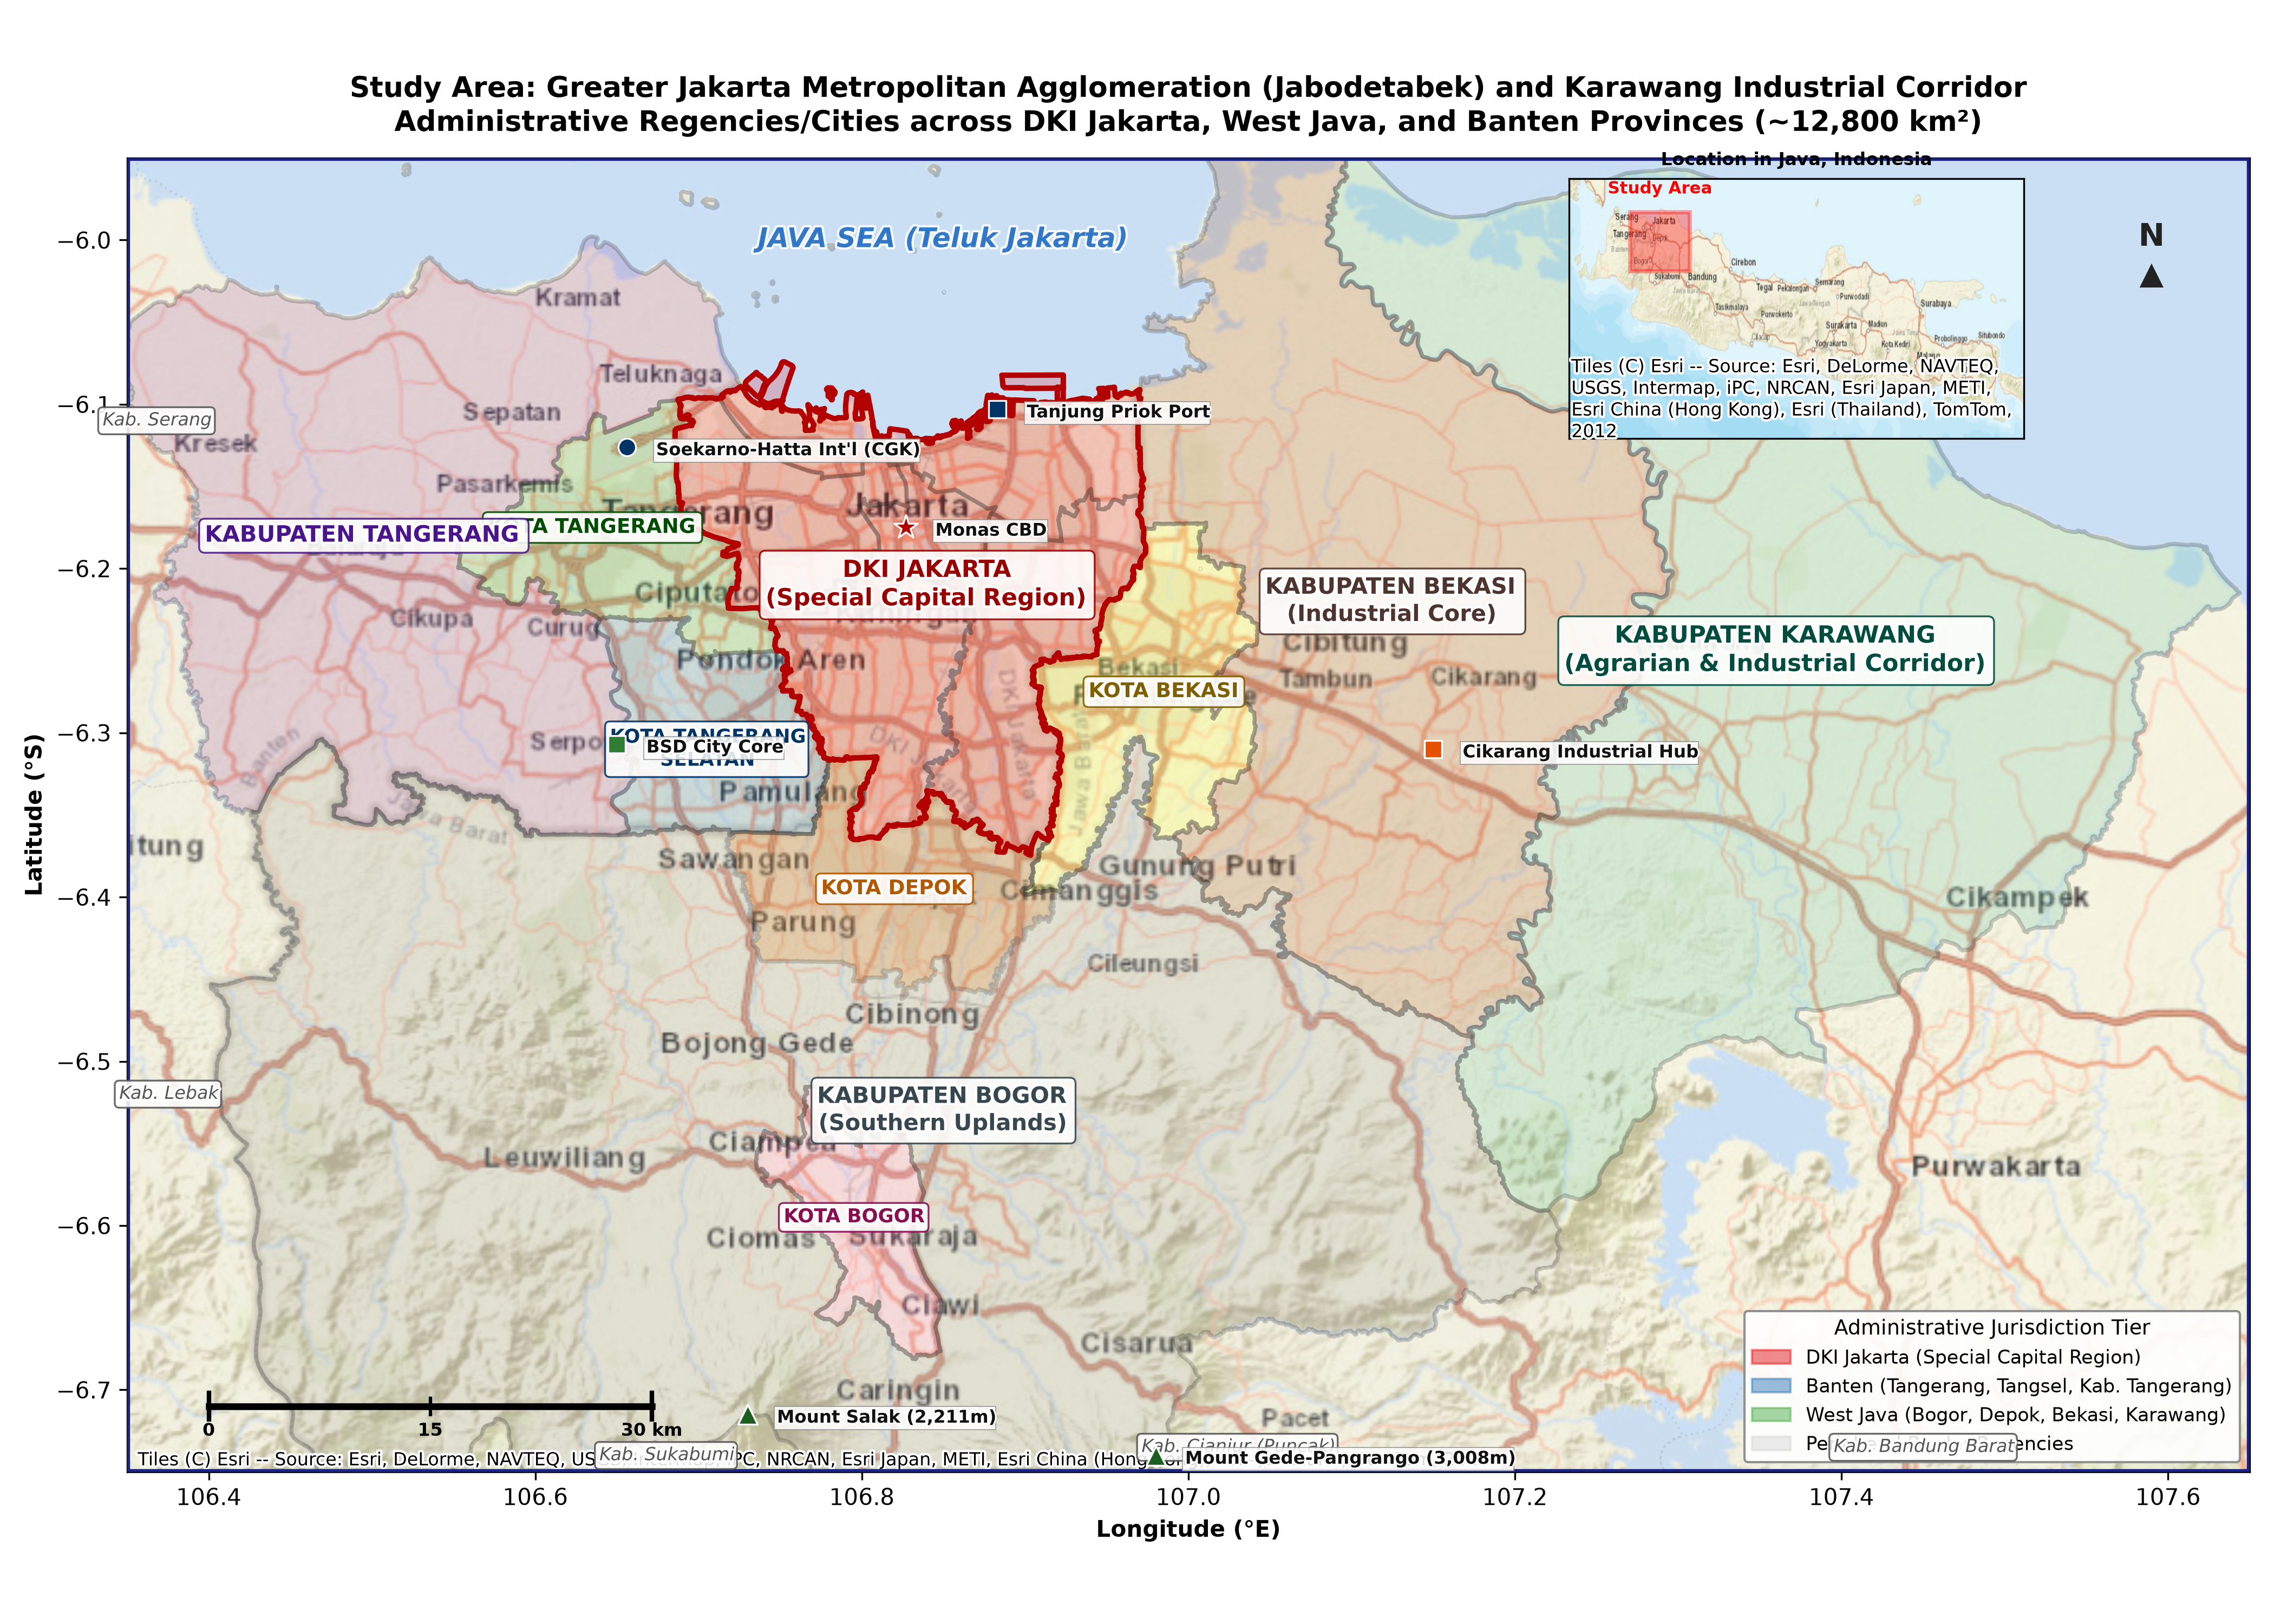
\includegraphics[width=0.96\textwidth]{figures/study_area_map.png}
\caption{Regional setting across Greater Jakarta (\textit{Jabodetabek}) and Karawang Regency ($\approx 12,800\text{ km}^2$), showing provincial and municipal boundaries across DKI Jakarta, Banten, and West Java along with major ports, commercial cores, and upland terrain.}
\label{fig:study_area_map}
\end{figure}

To avoid administrative boundary distortions \citep{Openshaw1984}, spatial layers are aggregated onto an Uber H3 Resolution-8 grid \citep{Sahr2003}, where each hexagon spans $\approx 0.737\text{ km}^2$ ($73.73\text{ ha}$; edge length $\approx 531\text{ m}$). Confined urban-extent masks intersect GHSL Settlement Model (\texttt{GHS-SMOD}) urban classes ($\{21, 22, 23, 30\}$) with cells containing at least one non-industrial residential footprint, restricting baselines and inequality metrics to built-up neighborhoods without relying on \texttt{GHS-POP}.

\subsection{Vetted Open Dataset Inventory}
Following Section~2's vetting criteria, only global open datasets that avoid coarse block smearing, circular population ratios, nightlight saturation, and service-proximity inversion enter the pipeline (Table~\ref{tab:dataset_inventory}). Disqualified layers---including \texttt{GHS-POP}, VIIRS nightlights, Sentinel-5P and $\text{PM}_{2.5}$ atmospheric grids, 1~km MODIS fallbacks, GLO-30 terrain slopes, flood layers, Overture/OSM service counts, and Meta's Relative Wealth Index---are excluded.

\begin{table}[htbp]
\centering
\caption{Vetted Open Global Datasets and Validation Labels Entering Preparation.}
\label{tab:dataset_inventory}
\footnotesize
\begin{tabularx}{\textwidth}{@{}>{\raggedright\arraybackslash}p{2.2cm}>{\raggedright\arraybackslash}p{3.0cm}>{\raggedright\arraybackslash}p{2.3cm}>{\raggedright\arraybackslash}p{2.0cm}>{\raggedright\arraybackslash}X@{}}
\toprule
\textbf{Group} & \textbf{Dataset} & \textbf{Source} & \textbf{Resolution} & \textbf{Role in Revised Pipeline} \\
\midrule
Spatial Grid & Uber H3 (Res 8) & Uber H3 & $0.737\text{ km}^2$ / $\approx 531\text{ m}$ edge & Equal-area spatial units and 6-neighbor adjacency graph for baselines and GAT-AE. \\
Built Footprints & Open Buildings (Google / Vida) & \citet{Sirko2021} & Sub-meter footprints & Small-footprint residential buildings ($<50$--$60\text{ m}^2$) and nearest-neighbor spacing. \\
Land-Use Mask & OpenStreetMap (2024-01-01) & Geofabrik / OSM & Vector polygons & Masks 21,135 non-residential zones (factories, ports, malls, offices) prior to built-form metrics. \\
Urban Envelope & EC JRC GHSL (BUILT / SMOD) & \citet{Pesaresi2024} & 10--100~m / 1~km & Urban extent mask for baselines and inequality; conditional residential share (\texttt{ghs\_res\_share}). \\
Optical Imagery & Copernicus Sentinel-2 L2A & ESA / GEE & 10~m VNIR & Cloud Score+ dry-season NDVI and candidate residential-masked 10~m GLCM roof texture. \\
Surface Heat & Landsat 8/9 C2 L2 (\texttt{ST\_B10}) & USGS / GEE & 100~m native (30~m grid) & Multi-year dry-season intra-urban surface heat anomaly ($\Delta\text{LST}$); no 1~km MODIS fallback. \\
Ground Truth & DKI Pergub 90 \& Karawang Kotaku & DKI / PUPR & RW / RT polygons & Validation labels only (438 DKI RWs \textit{KAT}~1--4; 100 stratified Karawang RTs); never model inputs. \\
\bottomrule
\end{tabularx}
\end{table}

\subsection{Masking, Compositing, and Feature Preparation Protocol}
Open layers pass through three standardized steps before single-indicator screening (Table~\ref{tab:feature_pool}):

\begin{enumerate}
    \item \textbf{Non-residential filtering and building geometry:} Footprints intersecting the 21,135 OSM non-residential zones are removed before computing small-footprint share ($<50\text{ m}^2$, paired with a $<60\text{ m}^2$ sensitivity check) and 25th-percentile nearest-neighbor centroid spacing (\texttt{res\_nn\_p25}). Because this building-footprint extract assigns a uniform 0.85 confidence score across polygons, confidence-threshold sensitivity sweeps cannot be run on it.
    \item \textbf{Multi-year 100~m thermal compositing and local baseline:} Single-season cloud masking over humid tropical cities leaves substantial thermal gaps; in preliminary 2023 dry-season extraction over Mainland DKI Jakarta, clear-sky 100~m Landsat 8/9 observations covered 55.8\% of cells while 25.3\% fell back to 1~km MODIS and 14.6\% remained missing. To prevent 1~km thermal smearing, we drop MODIS fallback completely and widen clear-sky Landsat 8/9 dry-season compositing progressively across 2023, 2022--2024, and 2021--2025 windows \citep{Voogt2003}. Intra-urban surface heat anomaly (\texttt{dlst\_local\_ring\_k5}) subtracts the median temperature of urban-masked neighbors within a $k=5$ hexagonal ring ($\approx 2.6\text{ km}$), pairing with a citywide urban-median baseline for sensitivity \citep{Chakraborty2019a, Stewart2012}.
    \item \textbf{Candidate roof-texture screening pool:} Full-resolution 10~m Sentinel-2 Cloud Score+ dry-season composites supply urban canopy greenness (\texttt{ndvi}) alongside residential-masked GLCM contrast and homogeneity (\texttt{s2\_res\_glcm\_*}, $3\times3$ window). Both texture metrics and \texttt{ghs\_res\_share} enter the candidate pool to be screened empirically against macro-density and official settlement records alongside the four core indicators.
\end{enumerate}

\begin{table}[htbp]
\centering
\caption{Candidate Feature Pool Prepared on H3 Resolution-8 Cells for Empirical Evaluation.}
\label{tab:feature_pool}
\footnotesize
\begin{tabularx}{\textwidth}{@{}>{\raggedright\arraybackslash}p{2.4cm}>{\raggedright\arraybackslash}p{3.2cm}>{\raggedright\arraybackslash}p{1.8cm}>{\raggedright\arraybackslash}X@{}}
\toprule
\textbf{Physical Domain} & \textbf{Variable Name} & \textbf{Status} & \textbf{Operational Definition} \\
\midrule
Built Form & \texttt{res\_share\_lt50} & \textbf{Core} & Share of masked residential footprints $<50\text{ m}^2$ ($<60\text{ m}^2$ sensitivity check). \\
Built Form & \texttt{res\_nn\_p25} & \textbf{Core} & 25th-percentile nearest-neighbor centroid distance (m) across masked residential roofs. \\
Built Form & \texttt{ghs\_res\_share} & \textbf{Conditional} & Residential share of built-up surface inside the urban extent (flags industrial encroachment). \\
Roof Texture & \texttt{s2\_res\_glcm\_*} & \textbf{Candidate} & Residential-masked 10~m Sentinel-2 GLCM contrast and homogeneity ($3\times3$ window; screened before selection). \\
Micro-Environment & \texttt{ndvi} & \textbf{Core} & Urban-masked 10~m Sentinel-2 dry-season canopy greenness. \\
Micro-Environment & \texttt{dlst\_local\_ring\_k5} & \textbf{Core} & Multi-year 100~m Landsat 8/9 LST minus $k=5$ urban-ring median (K; citywide median sensitivity). \\
\bottomrule
\end{tabularx}
\end{table}
